\documentclass[a4paper,12pt]{report}

\usepackage[T1]{fontenc}
\usepackage[utf8]{inputenc}
\usepackage[english]{babel}

\usepackage[hidelinks]{hyperref}
\usepackage{graphicx}
\usepackage{caption}
\usepackage{subcaption}

\title{Connector - Reference manual }
\author{Gianluigi Forte}

\usepackage{listings}
\usepackage{color}

\lstdefinelanguage{asymptote}{%
keywords=[1]{import, unitsize, add, shift,
 show, arc, include}, %pour asymptote + geometry
keywords=[2]{label, draw, dot, geometry, grid, triangleabc, perpendicularmark},% pour les autres extensions
keywords=[3]{pair, triangle, path}, % pour les classes
keywords=[4]{lightgray, black, gray, red}, %pour les couleurs
keywords=[5]{bp, pt, cm,  % unités
 N, E, S, W, NE, SE, SW, NW,
 NNE, ENE, ESE, SSE, SSW, WSW, WNW, NNW},% points cardinaux
comment=[l]{//},
otherkeywords={ -- , .. , :: , \^\^},
sensitive=true,
%morecomment=[s]{/*}{*/},
%string=[d]",
moredelim=*[s][\color{black}]{"}{"},
moredelim=**[s][\color{black}]{{$}{$}}
}


\lstset{%
language=asymptote,
keywordstyle=[1]\ttfamily\bfseries\color{black},
keywordstyle=[2]\ttfamily\color{black},
keywordstyle=[3]\ttfamily\bfseries,
keywordstyle=[4]\ttfamily\color{black},
keywordstyle=[5]\ttfamily\bfseries\color{black},
identifierstyle=\ttfamily\color{black},
firstnumber=5
}% à compléter au besoin
%
%

\begin{document}
\maketitle

\section*{Introduction}

Connector is a library written in \emph{Asymptote} language to generate figures of electronic schematics. \LaTeX and \emph{Asymptote}, differently from other programs like Word or Write, are languages designed to produce documents with the best quality outputs for prints or presentations starting from a description, of the content to be produced, expressed programmatically in a source code text file and then produced in output after the compilation process. The idea behind the \emph{connector} library is to provide a ready to use set of functions written in Asymptote language to draw electrical components, link them with connection (wires), decorate with labels and produce the output figure as pdf or png files to be embedded in a larger Latex document or any kind of other usage like websites, videos, presentations and so on. An example of the image generated with \emph{connector} is shown in figure \ref{threePhaseInverterExample}. The source code \texttt{ThreePhaseInverter.asy} to produce the figure is included in the library.

\begin{figure}[ht]
  \centering
  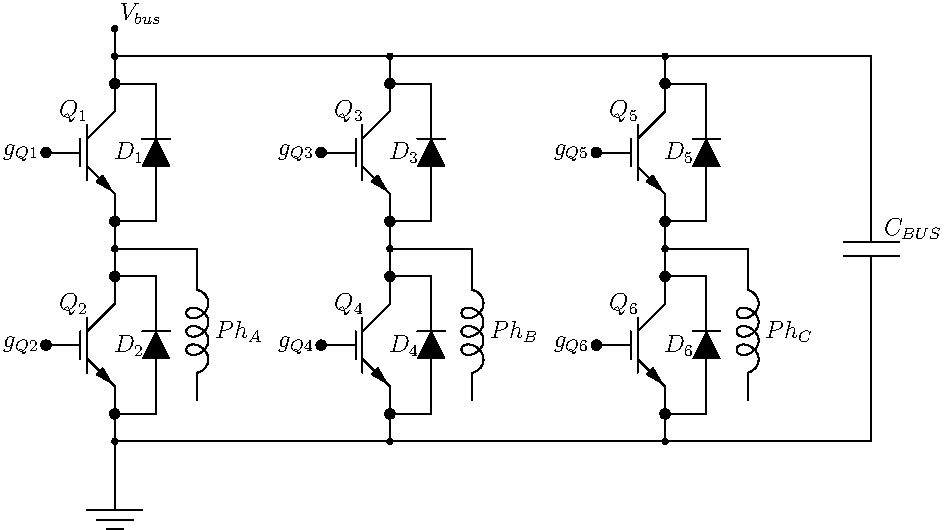
\includegraphics[width=1.0\textwidth]{ThreePhaseInverter.pdf}
  \caption{Example of schematics generated with \emph{connector}}
  \label{threePhaseInverterExample}
\end{figure}

\section*{Electronic Symbols}

The following list of components have been included in the libary and can be used out-of-the-box: node, resistor, capacitor, inductor, fuse, diode, relay, relay SPDT, IGBT, MOS, power ground, signal ground. Maybe other will be added in the future, if you want to collaborate to add other symbols please let me know at \emph{\href{mailto:koalakoker@gmail.com}{koalakoker@gmail.com}}.

In the figures from \ref{nodeInfo} to \ref{gndSignalInfo} are shown the components, the anchor points as a black dot. The anchor point direction is indicated with a green line starting from the dot and going outward, the anchor point index number is indicated near the end of the green line. It is also indicated the position of the pivot point $(0,0)$ and and also the position of the $(1,0)$ point for a spatial reference; both are indicated with a red crosses.

In figure \ref{nodeInfo} is shown a generic node symbol. See \texttt{nodeInfo.asy} code to reproduce the figure. Note that this symbol have four anchor points going in four different directions. It can be very useful to connect different part of the schematics with a connector line.

To draw any symbol without the indication of the anchor points, pivot point and all other info simply call the \texttt{draw} method without the \texttt{drawOpt} parameter or setting it to \texttt{null}.   

\begin{figure}[ht]
\centering
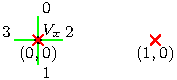
\includegraphics[width=0.5\textwidth]{nodeInfo}
\caption{Generic node symbol}
\label{nodeInfo}
\end{figure}

In figure \ref{resistorInfo} is shown the resistor symbol. See \texttt{resistorInfo.asy} code to reproduce the figure.

\begin{figure}[ht]
\centering
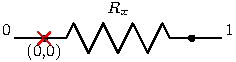
\includegraphics[width=0.5\textwidth]{resistorInfo}
\caption{Resistor symbol}
\label{resistorInfo}
\end{figure}

In figure \ref{capaciorInfo} is shown the capacitor symbol. See \texttt{capaciorInfo.asy} code to reproduce the figure.

\begin{figure}[ht]
\centering
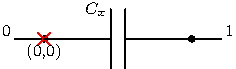
\includegraphics[width=0.5\textwidth]{capacitorInfo}
\caption{Capacitor symbol}
\label{capaciorInfo}
\end{figure}

In figure \ref{inductorInfo} is shown an inductor symbol. See \texttt{inductorInfo.asy} code to reproduce the figure.

\begin{figure}[ht]
\centering
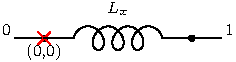
\includegraphics[width=0.5\textwidth]{inductorInfo}
\caption{Inductor symbol}
\label{inductorInfo}
\end{figure}

In figure \ref{fuseInfo} is shown the fuse symbol. See \texttt{fuseInfo.asy} code to reproduce the figure.

\begin{figure}[ht]
\centering
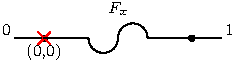
\includegraphics[width=0.5\textwidth]{fuseInfo}
\caption{Fuse symbol}
\label{fuseInfo}
\end{figure}

In figure \ref{diodeInfo} is shown the diode symbol. See \texttt{diodeInfo.asy} code to reproduce the figure.

\begin{figure}[ht]
\centering
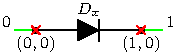
\includegraphics[width=0.5\textwidth]{diodeInfo}
\caption{Diode symbol}
\label{diodeInfo}
\end{figure}

In figure \ref{relayInfo} is shown the relay symbol. See \texttt{relayInfo.asy} code to reproduce the figure.

\begin{figure}[ht]
\centering
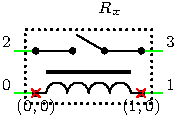
\includegraphics[width=0.45\textwidth]{relayInfo}
\caption{Relay symbol}
\label{relayInfo}
\end{figure}

In figure \ref{relaySPDTInfo} is shown the relay SPDT symbol. See \texttt{relaySPDTInfo.asy} code to reproduce the figure.

\begin{figure}[ht]
\centering
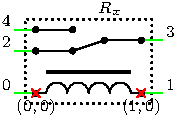
\includegraphics[width=0.45\textwidth]{relaySPDTInfo}
\caption{Relay SPDT symbol}
\label{relaySPDTInfo}
\end{figure}

In figure \ref{igbtInfo} is shown the IGBT symbol. See \texttt{igbtInfo.asy} code to reproduce the figure.

\begin{figure}[ht]
\centering
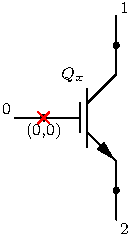
\includegraphics[width=0.4\textwidth]{igbtInfo}
\caption{Igbt symbol}
\label{igbtInfo}
\end{figure}

In figure \ref{mosInfo} is shown the MOSFET transistor symbol. See \texttt{mosInfo.asy} code to reproduce the figure.

\begin{figure}[ht]
\centering
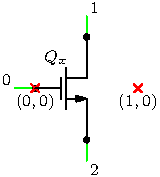
\includegraphics[width=0.4\textwidth]{mosInfo}
\caption{MOSFET transistor symbol}
\label{mosInfo}
\end{figure}

In figure \ref{gndPowerInfo} is shown the power ground symbol. See \texttt{gndPowerInfo.asy} code to reproduce the figure.

\begin{figure}[ht]
\centering
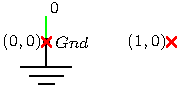
\includegraphics[width=0.4\textwidth]{gndPowerInfo}
\caption{Power ground symbol}
\label{gndPowerInfo}
\end{figure}

In figure \ref{gndSignalInfo} is shown the signal ground symbol. See \texttt{gndSignalInfo.asy} code to reproduce the figure.

\begin{figure}[ht]
\centering
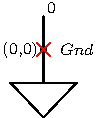
\includegraphics[width=0.4\textwidth]{gndSignalInfo}
\caption{Signal ground symbol}
\label{gndSignalInfo}
\end{figure}

\clearpage
\section*{Connectors}

It is possible to draw connectors (wires) between symbols with the function \texttt{drawAnchorConnector}. In particular the connection is done starting from one anchor point to another ancor point that are defined in the sybmol (see from figure \ref{nodeInfo} to figure \ref{gndSignalInfo} as reference). The path of the connector is automatically computed by the library in the best way and is drown according the direction of the ancor point. The figure \ref{connectorExample} show an example of connections between generic objects.

\begin{figure}[ht]
  \centering
  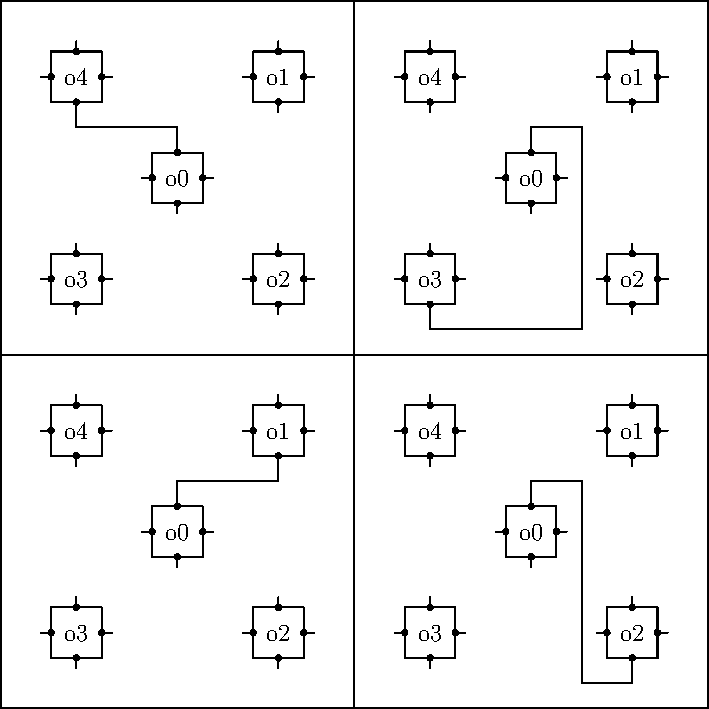
\includegraphics[width=1.0\textwidth]{N-S}
  \caption{Example of use of connectors between objects}
  \label{connectorExample}
\end{figure}

The \texttt{drawAnchorConnector} function takes as parameters respectively: the first object to be connected, the anchor point index of the first object, the second object to be connected and the index of the anchor point of the second object.

\texttt{drawAnchorConnector(obj1, Anchor1, obj2, Anchor2)}

There are also other three optional parameters that can be used to set the aspect of the connection ($r_1,r_2,r_3$). As shown in figure \ref{r1_connectorExample}, the $r_1$ parameter can be used to define the distance of the two corners of the connector line (and so the distance of the vertical line in figure \ref{r1_connectorExample}). The parameter $r_1$ defines the distance of the first corner of the connector line from the first object expressed in percentage of the distance of the two objects.

\begin{figure}
  \centering
  \begin{subfigure}{.33\textwidth}
    \centering
    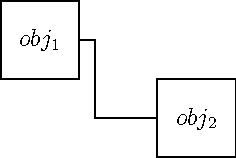
\includegraphics[width=0.9\linewidth]{connectorExample_r1_0_2.pdf}
    \caption{$r_1=0.2$}
    \label{fig:sfig1}
  \end{subfigure}\hfill
  \begin{subfigure}{.33\textwidth}
    \centering
    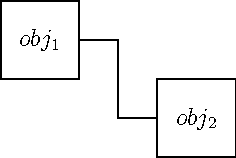
\includegraphics[width=0.9\linewidth]{connectorExample_r1_0_5.pdf}
    \caption{$r_1=0.5$}
    \label{fig:sfig2}
  \end{subfigure}\hfill
  \begin{subfigure}{.33\textwidth}
    \centering
    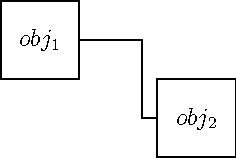
\includegraphics[width=0.9\linewidth]{connectorExample_r1_0_8.pdf}
    \caption{$r_1=0.8$}
    \label{fig:sfig3}
  \end{subfigure}

  \caption{Effect of $r_1$ parameter value on connector}
  \label{r1_connectorExample}
\end{figure}

The figure \ref{r2_connectorExample} shows the $r_2$ parameters. It affects the distance between the second object and the first corner of the connector line.

\begin{figure}
  \centering
  \begin{subfigure}{.33\textwidth}
    \centering
    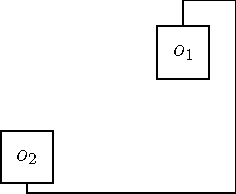
\includegraphics[width=0.9\linewidth]{connectorExample_r2_0_2.pdf}
    \caption{$r_2=0.2$}
  \end{subfigure}\hfill
  \begin{subfigure}{.33\textwidth}
    \centering
    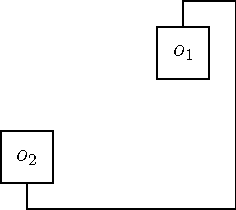
\includegraphics[width=0.9\linewidth]{connectorExample_r2_0_5.pdf}
    \caption{$r_2=0.5$}
  \end{subfigure}\hfill
  \begin{subfigure}{.33\textwidth}
    \centering
    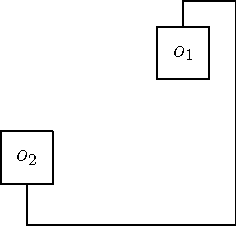
\includegraphics[width=0.9\linewidth]{connectorExample_r2_0_8.pdf}
    \caption{$r_2=0.8$}
  \end{subfigure}

  \caption{Effect of $r_2$ parameter value on connector}
  \label{r2_connectorExample}
\end{figure}

The figure \ref{r3_connectorExample} shows the $r_3$ parameters. It affects the distance between the first corner and the second corner (or equivalently the distance of the vertical bar) of the connector line.

\begin{figure}
  \centering
  \begin{subfigure}{.33\textwidth}
    \centering
    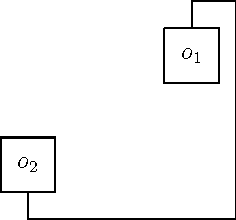
\includegraphics[width=0.9\linewidth]{connectorExample_r3_0_8.pdf}
    \caption{$r_3=0.8$}
  \end{subfigure}\hfill
  \begin{subfigure}{.33\textwidth}
    \centering
    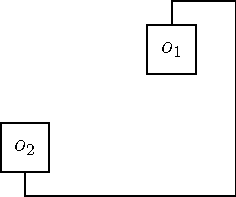
\includegraphics[width=0.9\linewidth]{connectorExample_r3_1_3.pdf}
    \caption{$r_3=1.3$}
  \end{subfigure}\hfill
  \begin{subfigure}{.33\textwidth}
    \centering
    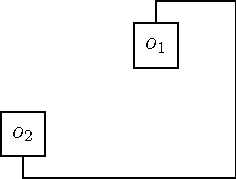
\includegraphics[width=0.9\linewidth]{connectorExample_r3_1_8.pdf}
    \caption{$r_3=1.8$}
  \end{subfigure}

  \caption{Effect of $r_2$ parameter value on connector}
  \label{r3_connectorExample}
\end{figure}

\end{document}